\subsubsection{Spannungsverstärkungen}
Die Werte zur Bestimmung der Spannungsverstärkungen wurden bei einer
Eingangsspannung von $U_{\mathrm{RMS}} = 1 \, \si{\volt}$ und einer
Frequenz von $f_e = 1 \, \si{\kilo\hertz}$ bestimmt. Der Lastwiderstand wurde
von $100 \, \si{\kilo\ohm}$ bis $1 \, \si{\kilo\ohm}$ variiert. Der interne Lastwiderstand beträgt $R_{\mathrm{L,intern}} =
100 \, \si{\kilo\ohm}$.


\begin{table}[H]
  \begin{center}
    \begin{tabular}{|c|c|c|c|}
      \hline
      $U_e / \si{\milli\volt}$ & $U_a / \si{\milli\volt}$ & $R_{\mathrm{L,gesamt}} / \si{\kilo\ohm}$ & $V_u$\\
      \hline
      \hline
      997.7 & 995 & 100 & 0.9973\\
      1020 & 994 & 33.33 & 0.9745\\
      1020 & 992 & 9.09 & 0.9726\\
      1000 & 918 & 0.99 & 0.918\\
      \hline
    \end{tabular}
  \end{center}
  \caption{RMS-Spannungswerte und daraus resultierende Verstärkung bei
    verscheidenen Lastwiderständen}
\end{table}

Die Messung am Oszilloskop war sehr verrauscht, weshalb sich unter Umständen
starke Abweichungen ergeben können.

\begin{figure}[H]
  \begin{center}
    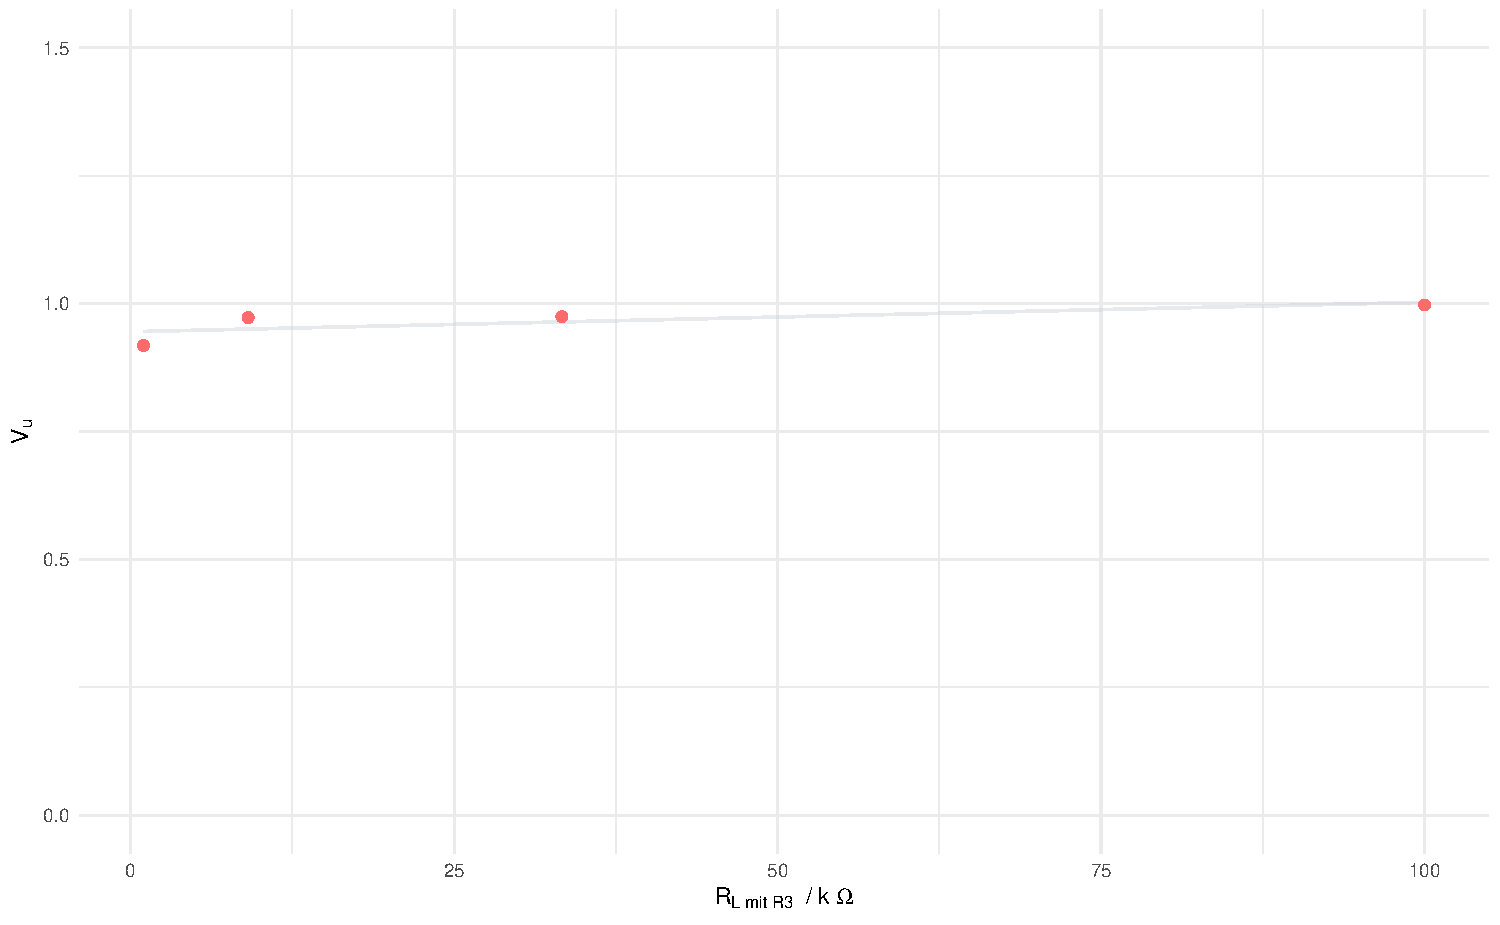
\includegraphics[width=\textwidth]{2_5/2_5_1.pdf}
  \end{center}
  \caption{Graph der Messwerte}
\end{figure}

Es lässt sich gut erkennen, dass die Verstärkereigenschaft der
Kollektorschaltung ($V_u \approx 1$) erfüllt ist.

\subsubsection{Eingangswiderstand}
Der theoretische Wert des Eingangswiderstandes der Kollektorschaltung ohne
Bootstrap, d.h. wenn $R_3 = 0$ und C weggelassen wird,  ist ( mit $B = 294$ im Arbeitspunkt)
\[r_{e,\mathrm{noBT}} = R_1 // R_2 // (B \cdot (R_4 // R_5)) = 184.5 \,\si{\kilo\ohm}\]

Messtechnisch konnte der Eingangsreihenwiderstand für die U/2 Methode nicht auf
einen ausreichend hohen Wert gestellt werden, da die verwendetete
Widerstandsdekade dies nicht hergab.

\subsubsection{Ausgangswiderstand}
Wie in den vorherigen Aufgaben ist der Ausgangswiderstand (bei einem
Lastwiderstand von $10 \, \si{\kilo\ohm}$)

\[r_a = R_L \left( \frac{U_{a0}}{U_{a1}} -1 \right)\]
\[r_a = 10 \, \si{\kilo\ohm} \left( \frac{995 \, \si{\milli\volt}}{993 \,
      \si{\milli\volt}} -1 \right)= 30.24 \, \si{\milli\ohm}\]

Der Ausgangswiderstand der Kollektorschaltung ohne Bootstrap, mit den gleichen
restlichen Widerstandswerten, ($I_C = 1.299 \, \si{\milli\ampere}$ (LTSPICE)) ist
\[r_a \approx \frac{1}{g_m} = \frac{U_T}{I_C} = \frac{26 \,
    \si{\milli\volt}}{1.299 \, \si{\milli\ampere}} = 20.02 \, \si{\ohm}\]